\chapter{Design \& Implementation} \label{chp:design_implementation}
This chapter explores the design and specific techniques used in this project.
We first look at the overall system architecture, and then dive deeper into the
chosen reinforcement learning algorithms, agents, neural networks, and
graphical user interface.

\section{Architecture}
This section describes the architectural design of the implementation. The
system consists of two overarching components: the graphical user interface
(GUI), and the Python notebooks used to train the models. There are two shared
folders used by both the user interface and training notebooks. Additionally,
there is a suite of utilities that is shared between all of the components,
\lstinline{utils.py}, for operations such as logging, file load and save
functions, and string processing functions.

We can see the connections between these components and the data flow in
\autoref{fig:project_schematic}; the filled arrowheads represent data flowing
in the specified direction, while the hollow arrowheads represent component and
function calls.

\begin{figure}[H]
  \centering
  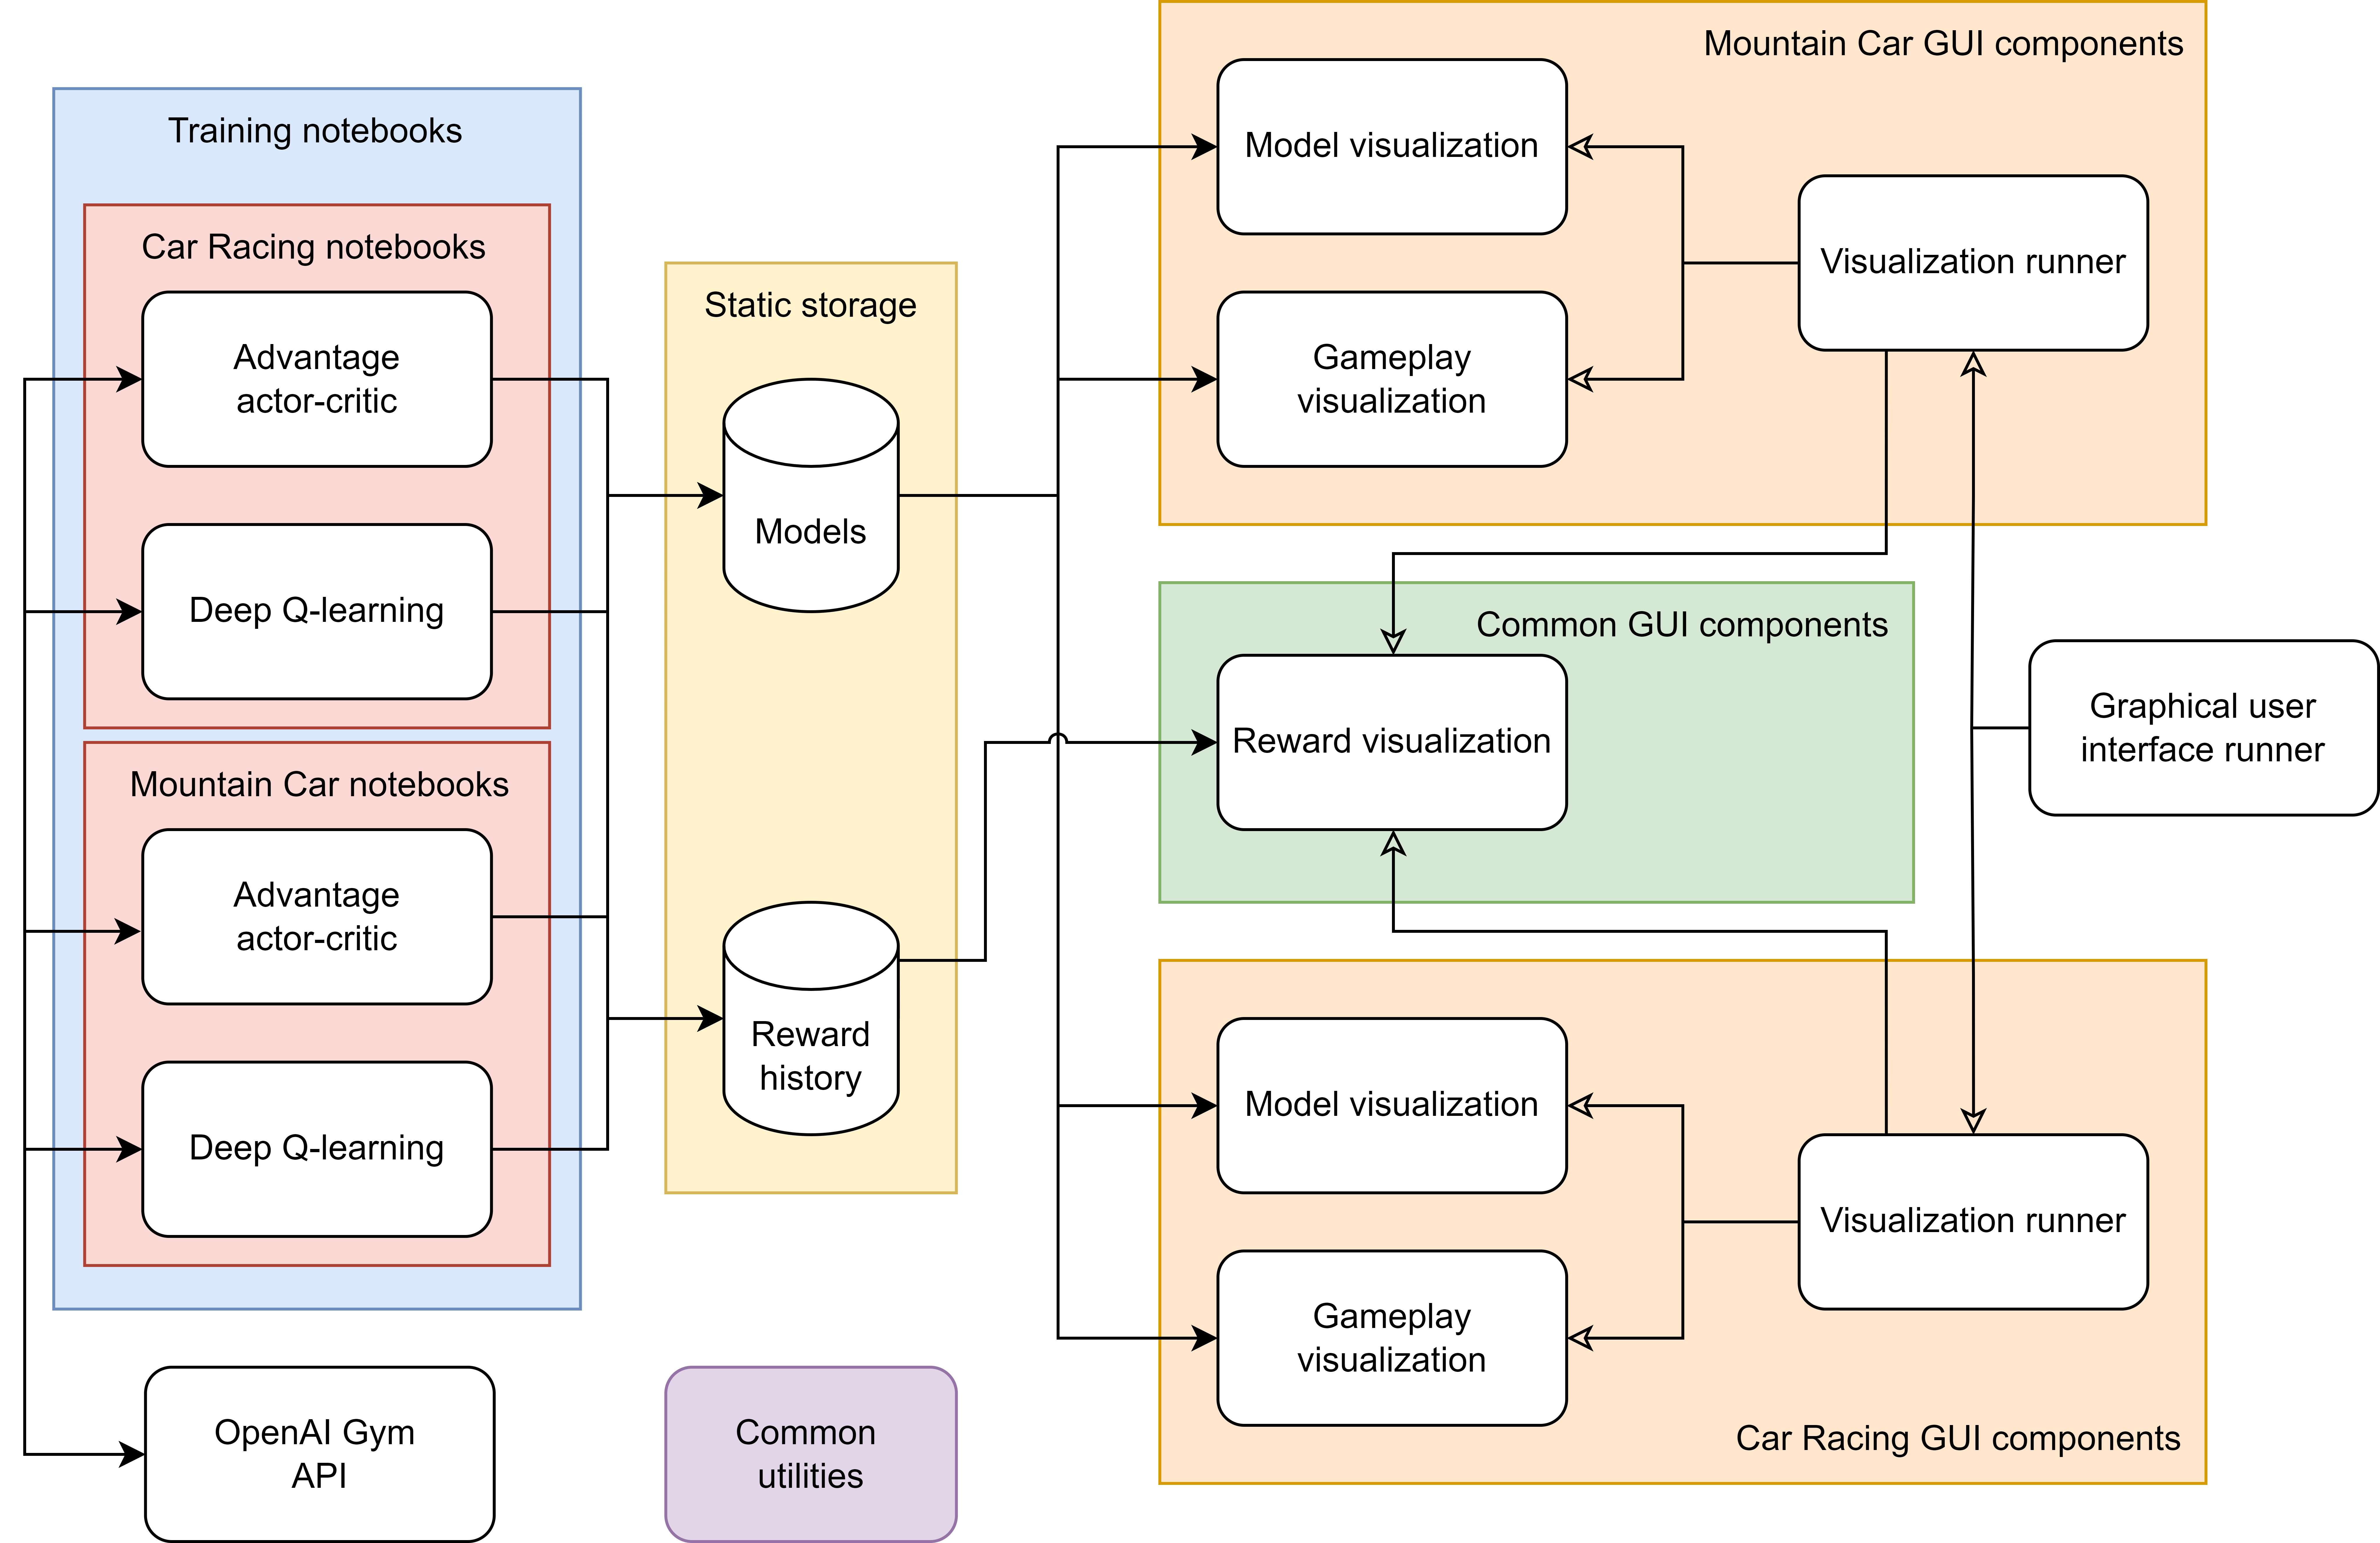
\includegraphics[width=1\textwidth]{figures/images/project_schematic.png}
  \caption[Project architecture schematic]{Schematic of the architecture of the project, showing the components and data flow between the training notebooks and GUI}
  \label{fig:project_schematic}
\end{figure}


\subsection{Training Notebooks}
As the name suggests, the training notebooks are used to train the agents;
there is a separate file for each game-agent pair, as that allows us to fine
tune the code for the relevant environment. The shared functions have been
abstracted to the utilities file, leaving only the core functionality of the
neural network and agent in the respective notebooks. These notebooks use
TensorFlow 2 to implement the neural networks, and they use the Gym API to
facilitate the agent's interactions with the environment; this process is
explained further in \autoref{sec:gym_environment}.

\subsection{Shared File Storage}
The training notebooks and user interface share two common storage folders:
\lstinline{models} and \lstinline{reward_history}. The Python notebooks produce
\lstinline{.h5} model files, which are the saved Keras models representing the
network's weights and any other data required to recreate the exact same model
when loaded. The notebooks also produce \lstinline{.npy} files, which contain a
numpy array of the total reward from every episode during training; this allows
us to plot visualizations containing a reward history graph with a slider to
control the rolling average window size.

\subsection{Graphical User Interface}
We have a master graphical user interface runner file, \lstinline{gui.py},
which calls separate user interface runners for each of the games; this was
required due to the differences between the games and therefore the differences
in network architectures. When the user selects a visualization, the
corresponding files read the required data from the shared folders and display
the selected visualization. This is described in further detail in
\autoref{sec:visualization_design}.

\subsection{Environment}

\subsubsection{Conda}
In order to ensure consistency and reliability during the development process,
we used a \lstinline{conda} environment to run the project. This allowed us to
install the required version of Python and the imported packages, without
interference from an existing Python installation on the machine.

\subsubsection{OpenAI Gym} \label{sec:gym_environment}

This project uses Gym, a Python toolkit developed by OpenAI that provides a
standardized environment for training and testing ML models. It also provides
implementations for both of the chosen games, and many more classic control
games and complex environments \cite{brockman2016gym}. The efficiency and
extensibility of this library allows us to focus on the implementation of the
neural networks and the experimentation of the hyperparameters.

The Python code in \autoref{lst:mountain_car_environment} shows basic usage of
the API to create and interact with the Mountain Car environment. The
environment is first initialized with the selected game, and it is reset for
each episode. We have the option to set a seed for testing to ensure equal
environments and starting states for both agents, although we would like
randomness during training for generalization in newly generated environments.
We pass the state to our agent, which then chooses an action. This is used to
step through the environment, until the game is solved, or the maximum number
of timesteps is reached, as described in \autoref{sec:mountain_car_background}
and \autoref{sec:car_racing_background}. After the episode is finished, the
environment is closed.

\begin{lstlisting}[style=codestyle, basicstyle=\ttfamily\footnotesize, caption={Using OpenAI Gym with the Mountain Car environment}, label=lst:mountain_car_environment]
import gym

EPISODES = 500

env = gym.make("MountainCar-v0")

for e in range(EPISODES):
    # Reset the environment and variables for each episode
    state = env.reset()
    t = 0
    done = False
    total_reward = 0

    while not done:
        # Randomly sample the action space
        action = env.action_space.sample()

        # Take the action
        next_state, reward, done, info = env.step(action)

        state = next_state
        total_reward += reward
        t += 1

    print(f"Episode {e+1} finished after {t} timesteps "
          f"with {total_reward} reward")

env.close()
\end{lstlisting}


Both environments use a discrete action space; this is a conscious decision, as
the DQN algorithm can't work with continuous action spaces, while A2C can.
Choosing discrete variations of the games instead of the continuous ones
ensures both algorithms are trained and tested under the exact same conditions.
Due to the difference in the input and output space of the games, separate
agents are used for each game.

Since one of the primary aims of this project is to decrease training time for
the neural networks, we set the hyperparameter for the maximum number of
episodes to 500.

\section{Deep Q-Learning}
As the name suggests, deep Q-learning is the combination of Q-learning with
deep neural networks; these networks are used as function approximators for the
Q-value function. \autoref{fig:q_vs_dq} shows the difference between both of
these techniques.

\begin{figure}[H]
  \centering
  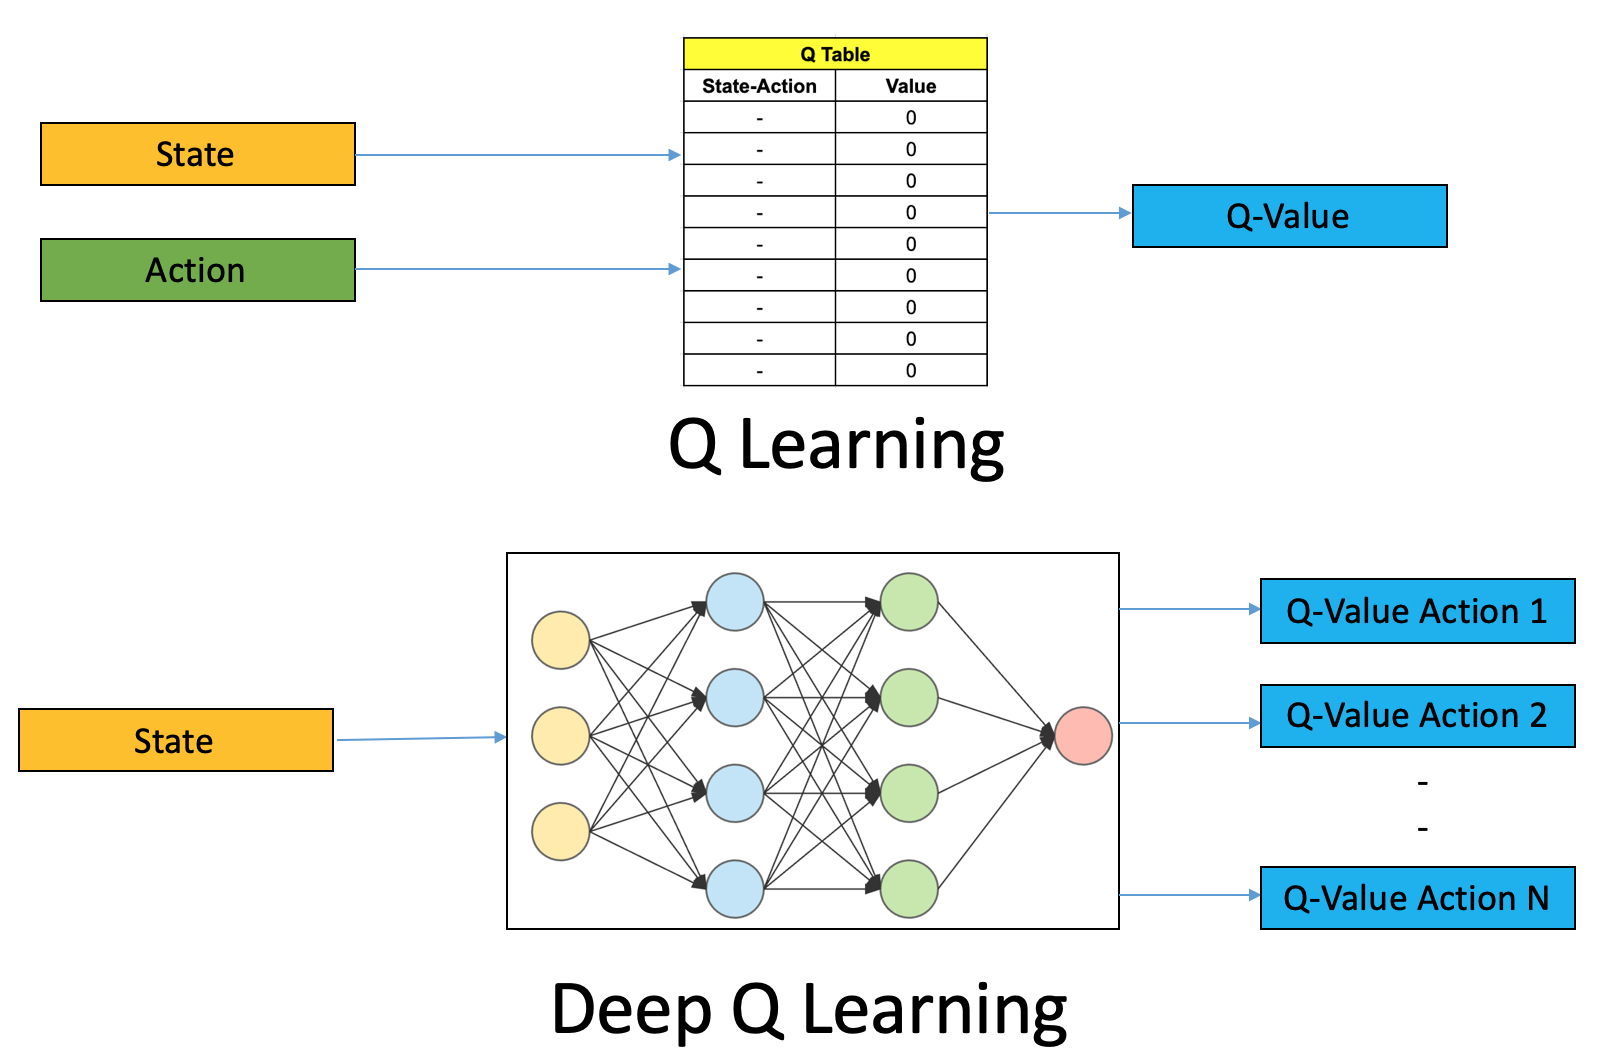
\includegraphics[width=0.7\textwidth]{figures/images/q_vs_dq.png}
  \caption[Q-learning vs deep Q-learning]{Comparison between Q-learning and deep Q-learning, showing their different structures and outputs  \cite{vidhya2019introduction}}
  \label{fig:q_vs_dq}
\end{figure}


\newpage

We use $\theta$ to represent the neural network's weights. We need to define a
loss function in order to update the weights and train the neural network.

\begin{definition}
  The \textit{loss function}
  $$L(\theta)=\mathbb{E}\left[\left(r_t+\gamma\cdot\max_{a_{t+1}}Q(s_{t+1},~a_{t+1};~\theta)-Q(s_{t},~a_{t};~\theta)\right)^{2}\right]$$
  \begin{itemize}[label={}]
    \item $Q(s_t,~a_t;~\theta)$, Q-value for state-action pair
    \item $r_t$, immediate reward
    \item $\gamma$, discount factor of future reward
    \item $\max\limits_{a_{t+1}} Q(s_{t+1},~a_{t+1};~\theta)$, estimate of optimal future reward for next state
  \end{itemize}
\end{definition}

The loss function is the same as the square of the TD error, defined in
\autoref{def:td_error_q_learning}. Taking the derivative of the loss function
with respect to the network weights gives us a gradient, which can be
optimized.

\begin{definition}
  The \textit{gradient}
  $$\frac{\partial{L(\theta)}}{\partial
      \theta}=\mathbb{E}\left[\left(r_t+\gamma\cdot\max_{a_{t+1}}Q(s_{t+1},~a_{t+1};~\theta)-Q(s_{t},~a_{t};~\theta)\right)\frac{\partial{Q(s_{t},~a_{t};~\theta)}}{\partial\theta}\right]$$
\end{definition}

\subsection{Epsilon Greedy} \label{sec:epsilon_greedy}
$\epsilon$-greedy is a commonly used exploration technique for balancing the exploration-exploitation
tradeoff in off-policy algorithms. The hyperparameter $\epsilon$ is used to
determine the probability with which the agent explores. An action $a$ is selected as follows:

$$
  a =
  \begin{cases}
    \underset{a~\in~A}{\arg\max}~Q(a) & \text{with probability } 1-\epsilon \\
    \text{a random action }           & \text{with probability } \epsilon
  \end{cases}
$$

The value of $\epsilon$ decays as the number of episodes increases; it
eventually reaches a lower bound value, where it stays for the rest of the
training process.

The idea behind decaying $\epsilon$ is that the agent becomes more confident in
its policy as training progresses, slowly reducing the need to choose random
actions. An example of a decay graph is shown in \autoref{fig:epsilon_decay}.

\begin{figure}[H]
  \centering
  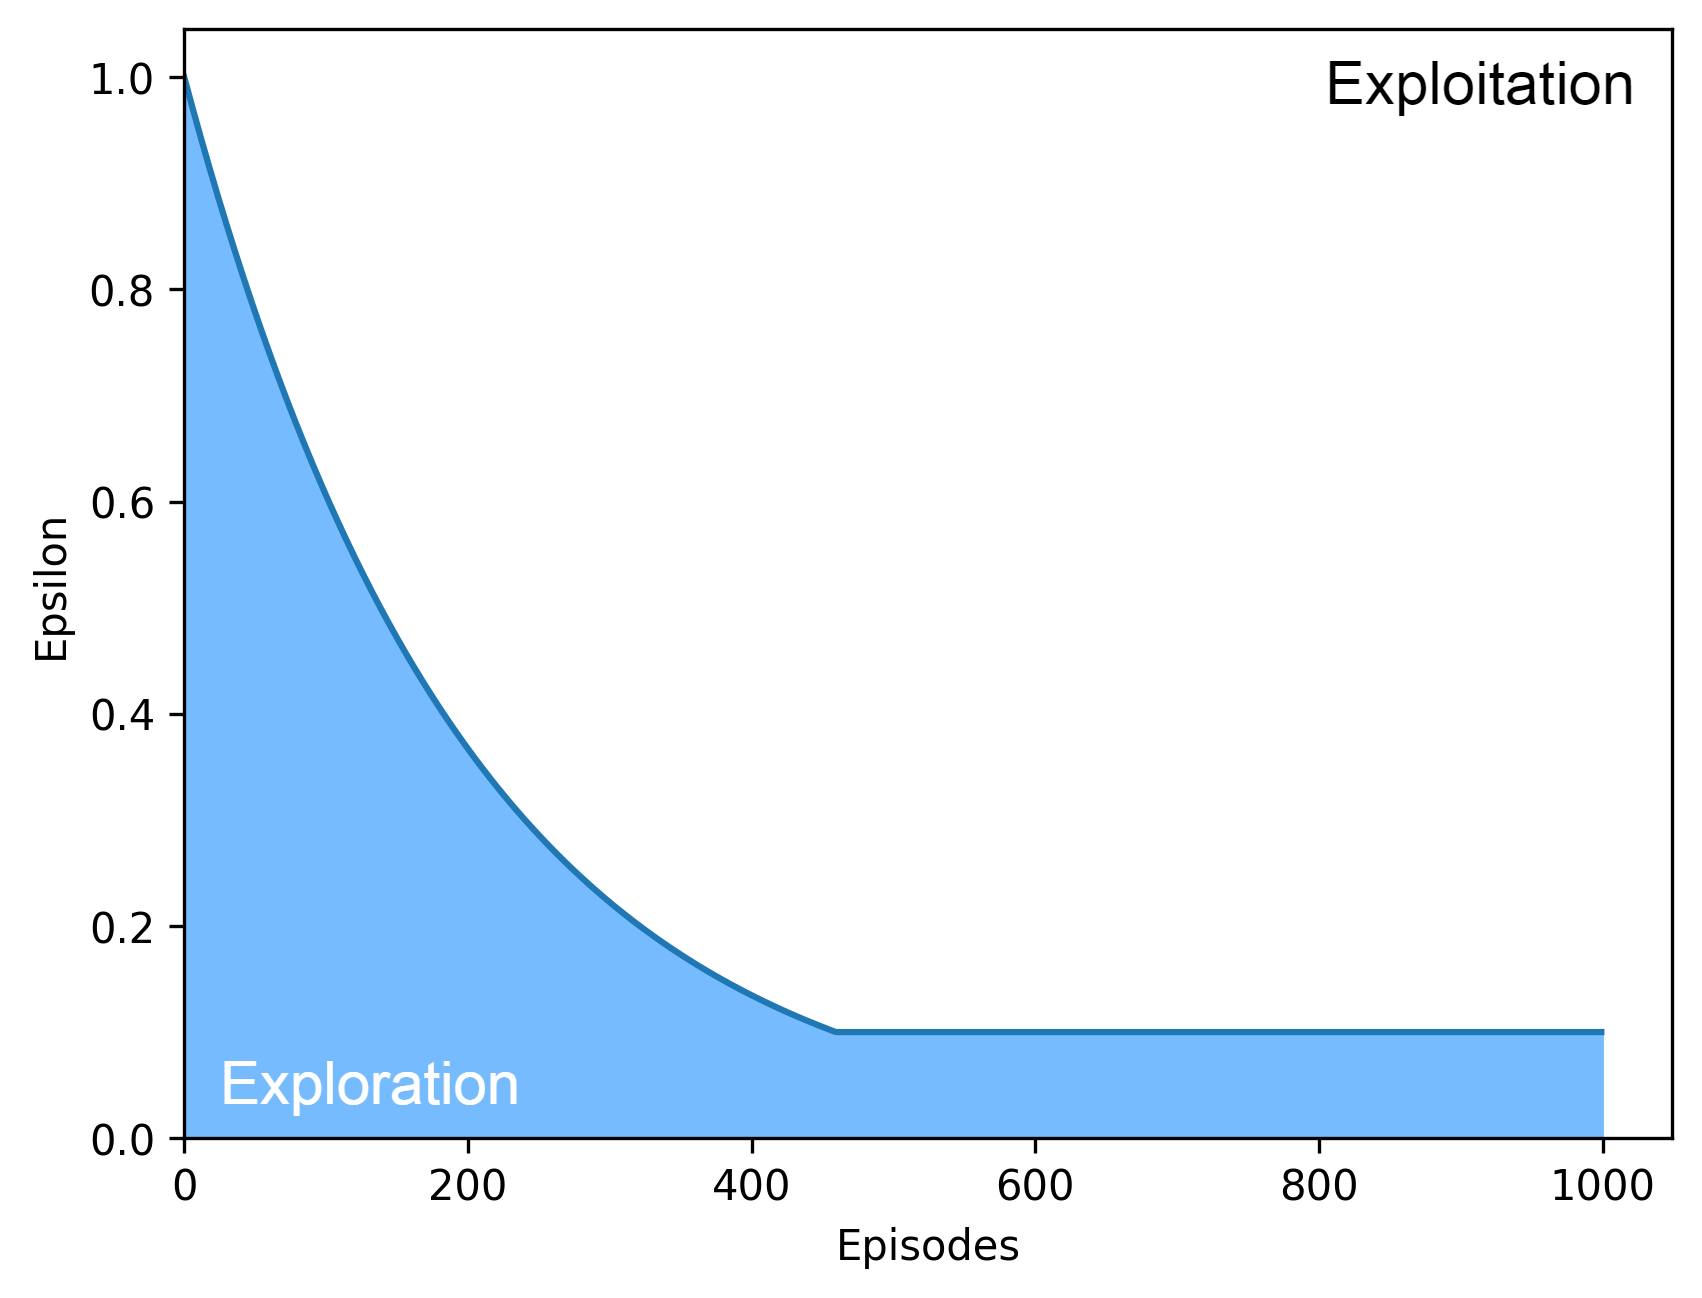
\includegraphics[width=0.6\textwidth]{figures/images/epsilon_decay.png}
  \caption[Epsilon decay graph]{Graph showing an $\epsilon$-decay multiplier of 0.995 every episode with minimum $\epsilon=0.1$, over 1000 episodes}
  \label{fig:epsilon_decay}
\end{figure}


\subsection{Experience Replay} \label{sec:experience_replay}

Experience replay is a technique used to improve the efficiency and stability
of the training process. Instead of using each experience\footnote{Experience
  refers to a transition from one state to another, and the associated action and
  reward} only once, this technique involves storing the agent's experiences in a
replay buffer $\mathcal{D}$. These experiences are then uniformly sampled in
minibatches during training, $U(\mathcal{D})$, which allows the agent to learn
from experiences that occurred in different parts of the state space, helping
with the network's generalization for new situations as it is not simply
learning from successive experiences. Improving generalization also helps with
the moving targets problem, described in earlier in
\autoref{sec:on_vs_off_policy}. We can provide an updated definition for our
loss function, incorporating experience replay.

\begin{definition}
  The \textit{loss function with experience replay}
  $$L(\theta)=\mathbb{E}_{(s_t,~a_t,~r_t,~s_{t+1})~\thicksim ~U(\mathcal{D})}\left[\left(r_t+\gamma\cdot\max_{a_{t+1}}Q(s_{t+1},~a_{t+1};~\theta)-Q(s_{t},~a_{t};~\theta)\right)^{2}\right]$$
\end{definition}

This project implements uniformly sampled experience replay, the technique
described above, as it provides excellent results \cite{mnih2013playing}. There
are many advanced variations of experience replay, including prioritized
experience replay \cite{schaul2015prioritized} and hindsight experience replay
\cite{andrychowicz2017hindsight}, which optimize this method further.

Below, we can see both a schematic and code implementation of the deep Q
learning algorithm, including all of the aforementioned improvements.

\begin{figure}[H]
  \centering
  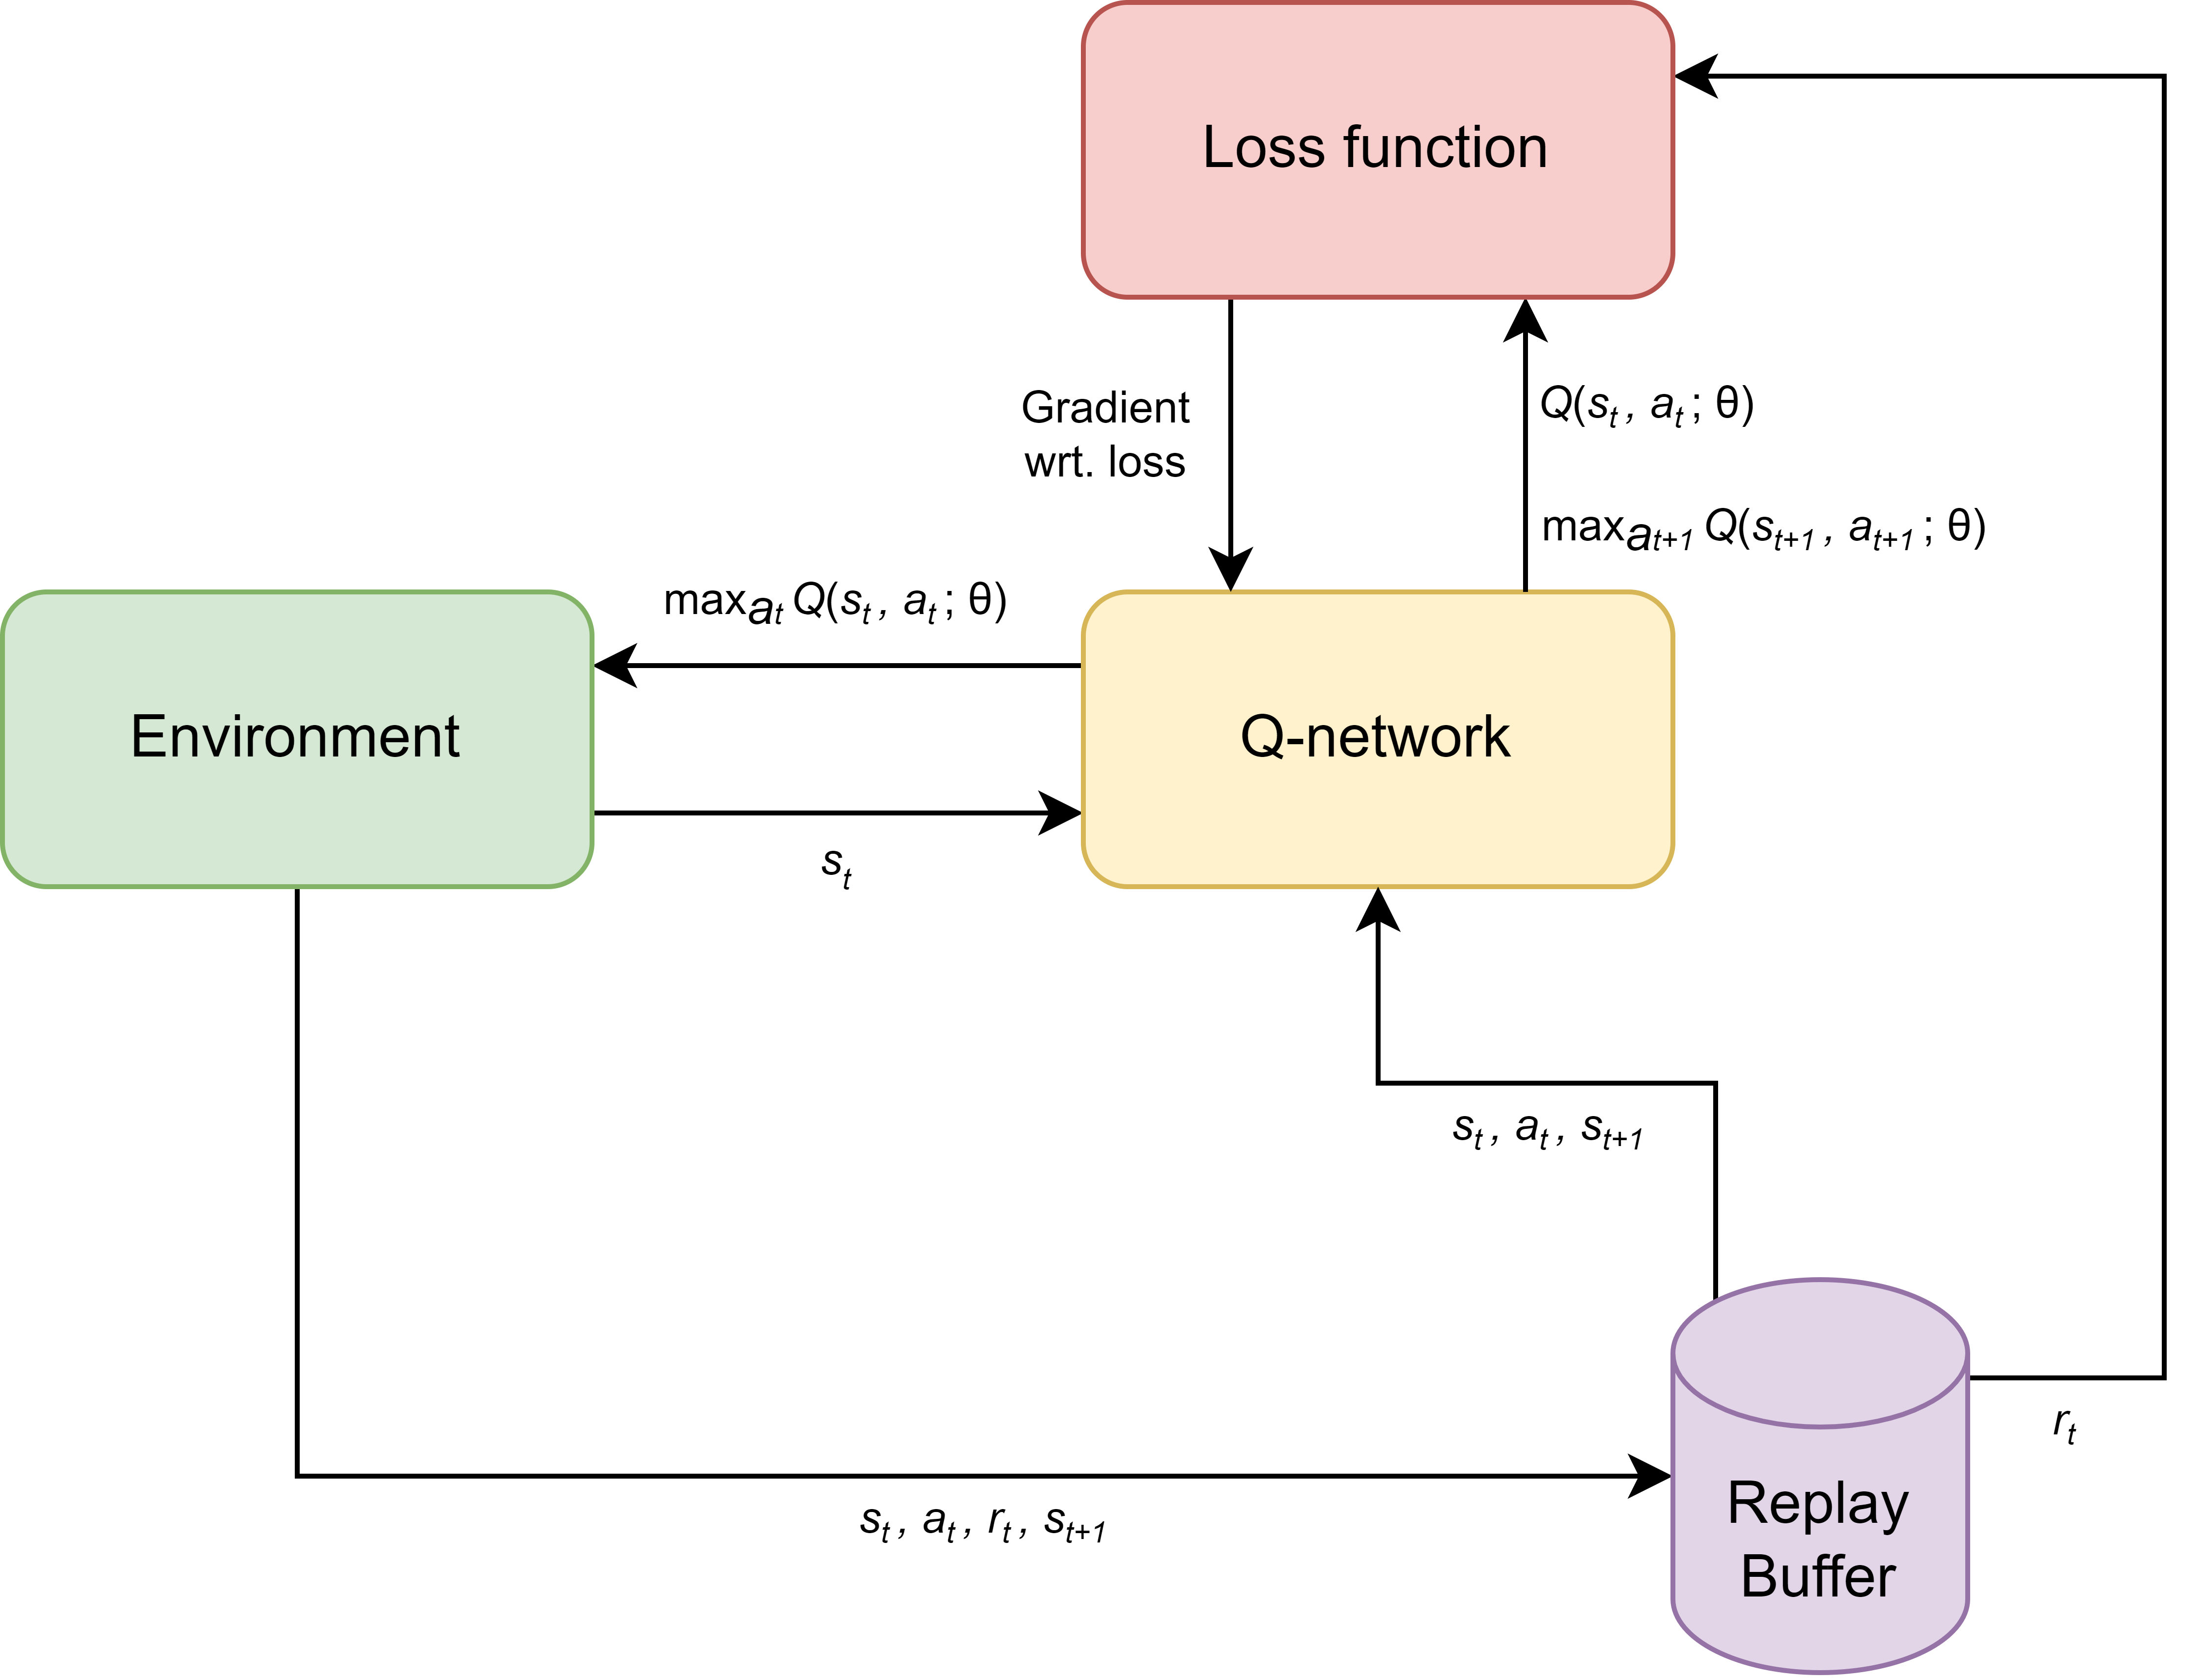
\includegraphics[width=0.8\textwidth]{figures/images/dqn_architecture.png}
  \caption[Deep Q-learning architecture]{Components and their interactions in the deep Q-learning algorithm with experience replay}
  \label{fig:dqn_architecture}
\end{figure}


\begin{algorithm}[H]
  \caption[Deep Q-Learning]{Deep Q-Learning with Experience Replay}
  \label{alg:deep_q_learning}
  \begin{algorithmic}
    \State Initialize Q-network with random weights $\theta$
    \For{episode $i$ in $1:N$}
    \State Set initial state $s_t$
    \While{$s_t$ is not terminal}
    \State{
      $
        a_t =
        \begin{cases}
          \max\limits_{a_t} Q(s_t, a_t;~\theta) & \text{with probability } 1-\epsilon \\
          \text{a random action }               & \text{with probability } \epsilon
        \end{cases}
      $
    }
    \State Take action $a_t$ and observe reward $r_t$ and new state $s_{t+1}$
    \State Store transition $(s_t,~a_t,~r_t,~s_{t+1})$ in $\mathcal{D}$
    \State Sample a random batch of transitions $(s_j,~a_j,~r_j,~s_{j+1})$ from $\mathcal{D}$
    \State{
      $
        y_j =
        \begin{cases}
          r_j                                                              & \text{for terminal } s_{j+1}     \\
          r_j +\gamma\cdot\max\limits_{a_{j+1}}Q(s_{j+1},~a_{j+1};~\theta) & \text{for non-terminal } s_{j+1}
        \end{cases}
      $
    }
    \State Perform gradient descent on $(y_j - Q(s_j,a_j;~\theta))^2$ wrt. the network weights $\theta$
    \State Update state $s_t \gets s_{t+1}$
    \EndWhile
    \EndFor
  \end{algorithmic}
\end{algorithm}


\newpage

\section{Advantage Actor-Critic}

Advantage actor-critic (A2C) is an instance of the actor-critic method, using
neural networks to approximate the actor and critic functions. We make some
improvements to the generic one-step actor-critic algorithm, by using entropy
regularization to encourage exploration, discussed in
\autoref{sec:entropy_regularization}. A2C was chosen due to its stability and
sample-efficiency compared to similar algorithms, such as Asynchronous
Advantage Actor-Critic (A3C) \cite{wu2017scalable}. We can define an advantage
function, which in the case of the one-step algorithm is equivalent to the TD
error in \autoref{def:td_error_actor_critic}.

\begin{definition} \label{def:td_error_a2c}
  The \textit{advantage}
  $$A(s_t, a_t) = r_t+\gamma\cdot V(s_{t+1}) - V(s_t)$$
  \begin{itemize}[label={}]
    \item $r_t$, immediate reward
    \item $\gamma$, discount factor of future reward
          \begin{itemize}[label={}]
            \item $\gamma\in[0,1]$
          \end{itemize}
    \item $V(s_t)$, estimate of cumulative reward from current state
    \item $V(s_{t+1})$, estimate of cumulative reward from next state
  \end{itemize}
\end{definition}

We can use this advantage function to compute the losses for both the actor and
the critic.

\begin{definition}
  The \textit{actor loss function}
  $$L_{actor}=-\log (\pi(a_t~|~s_t)) \cdot A(s_t, a_t)$$
\end{definition}

\begin{definition}
  The \textit{critic loss function}
  $$L_{\text{critic}} = A(s_t, a_t)^2$$
\end{definition}

\subsection{Stochastic Policy Exploration}
By using a stochastic policy rather than the deterministic variant, we
encourage the agent to explore, as we select an action based on the weighted
probability rather than taking the action with the maximum probability, like in
the Q-learning methods. The policy is initialized with random values, allowing
this technique to increase the probability of the agent exploring with new
state-action pairs in the beginning of the training process.

\subsection{Entropy Regularization} \label{sec:entropy_regularization}
Entropy regularization further encourages exploration by adding an entropy term
to the loss function of the actor, which is derived from the probability
distribution over the actions. This entropy term "flattens" the distribution,
forcing exploration by increasing the chances of an action with a lower
probability according to the actor network being chosen.

\begin{definition}
  The \textit{entropy} of the policy distribution
  $$H_t=-\log(\pi(a_t~|~s_t)) \cdot \pi(a_t~|~s_t)$$
\end{definition}

\begin{definition}
  The \textit{actor loss function with entropy regularization}
  $$L_{actor}=-\log (\pi(a_t~|~s_t)) \cdot A(s_t, a_t) - \beta\cdot H_t$$
\end{definition}

$\beta$ represents the entropy coefficient; a value of 0 means that no entropy regularization is used. As we increase this value, we increase the amount of regularization applied. The factor
is a hyperparameter optimized during training, with common values being
$\beta\in[0.01,0.50]$. We can see a visual representation of this in \autoref{fig:entropy_regularization}.

\begin{figure}[H]
  \captionsetup[subfigure]{justification=centering}
  \centering
  \begin{subfigure}[t]{0.47\linewidth}
    {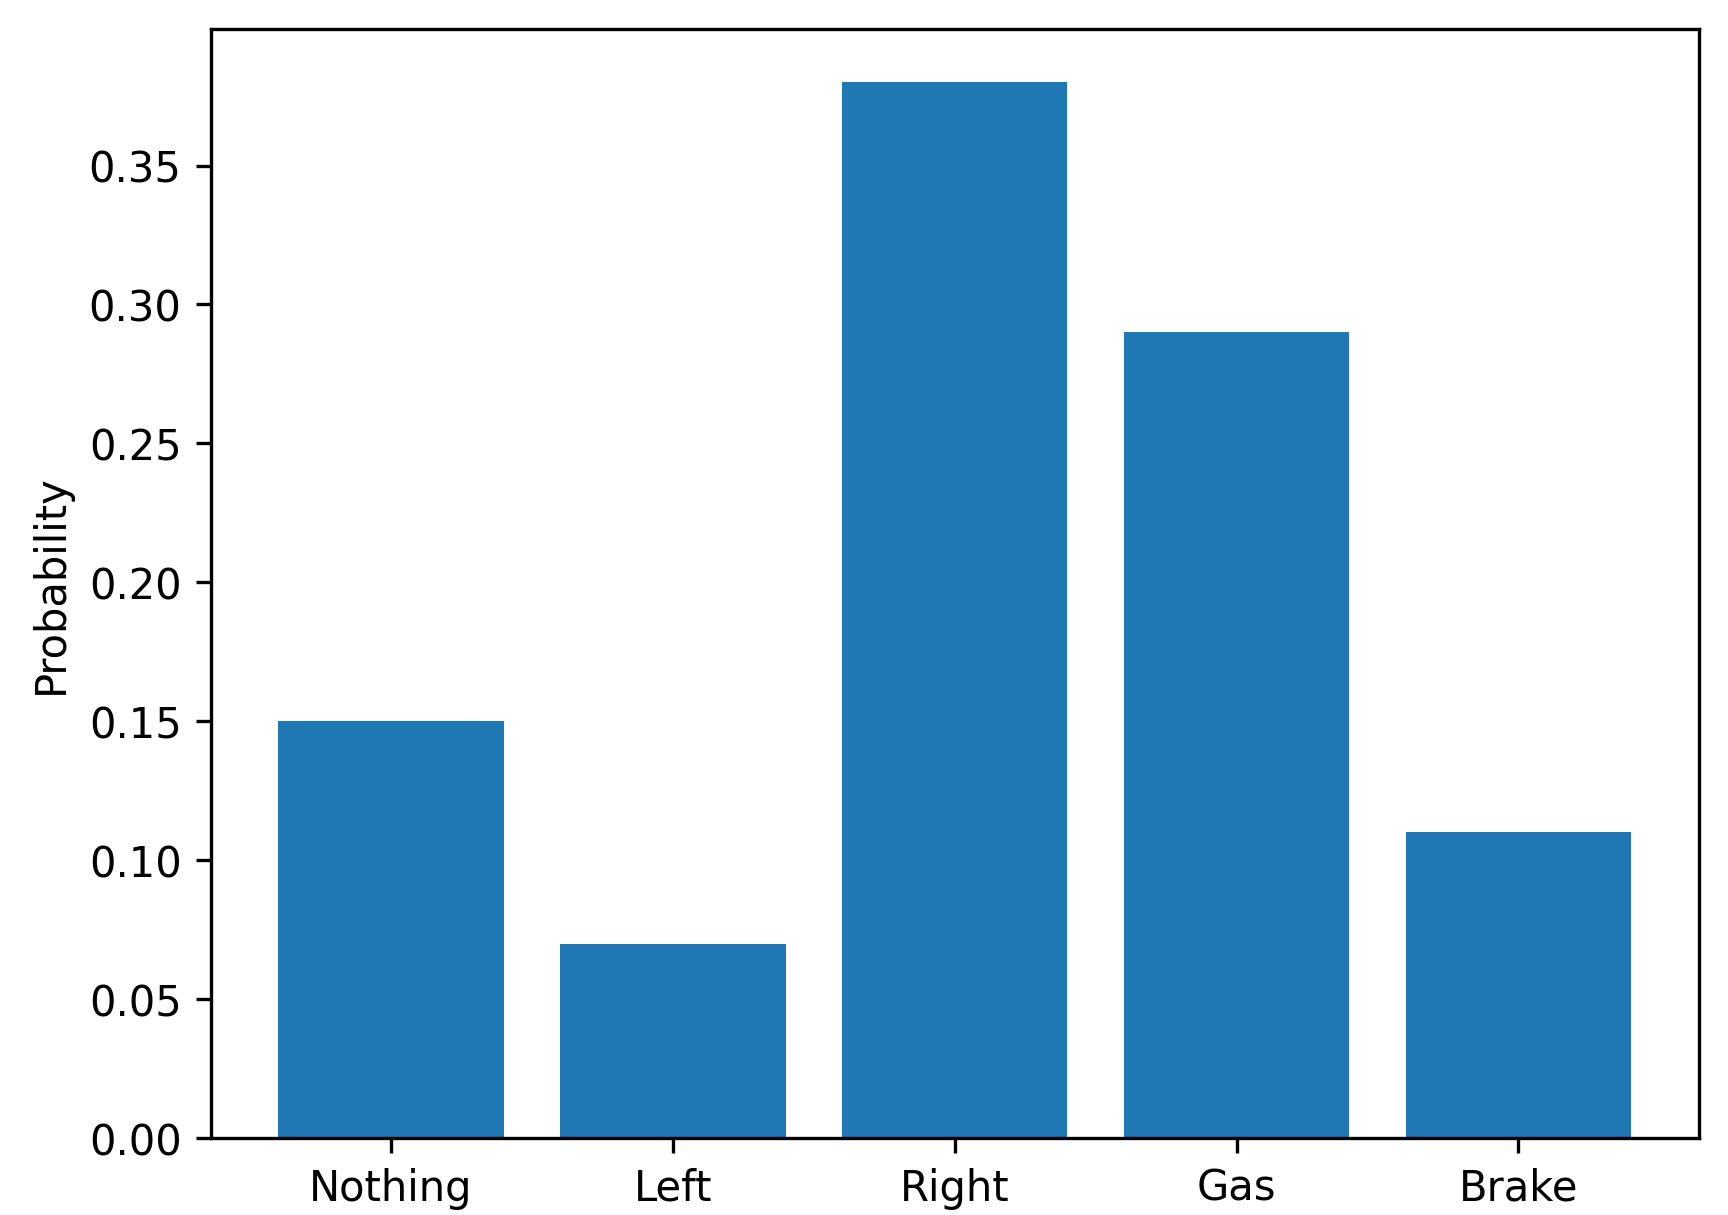
\includegraphics[height=5cm]{figures/images/unregularized.png}}
    \caption{Without regularization}
  \end{subfigure}
  \hfill
  \begin{subfigure}[t]{0.47\linewidth}
    {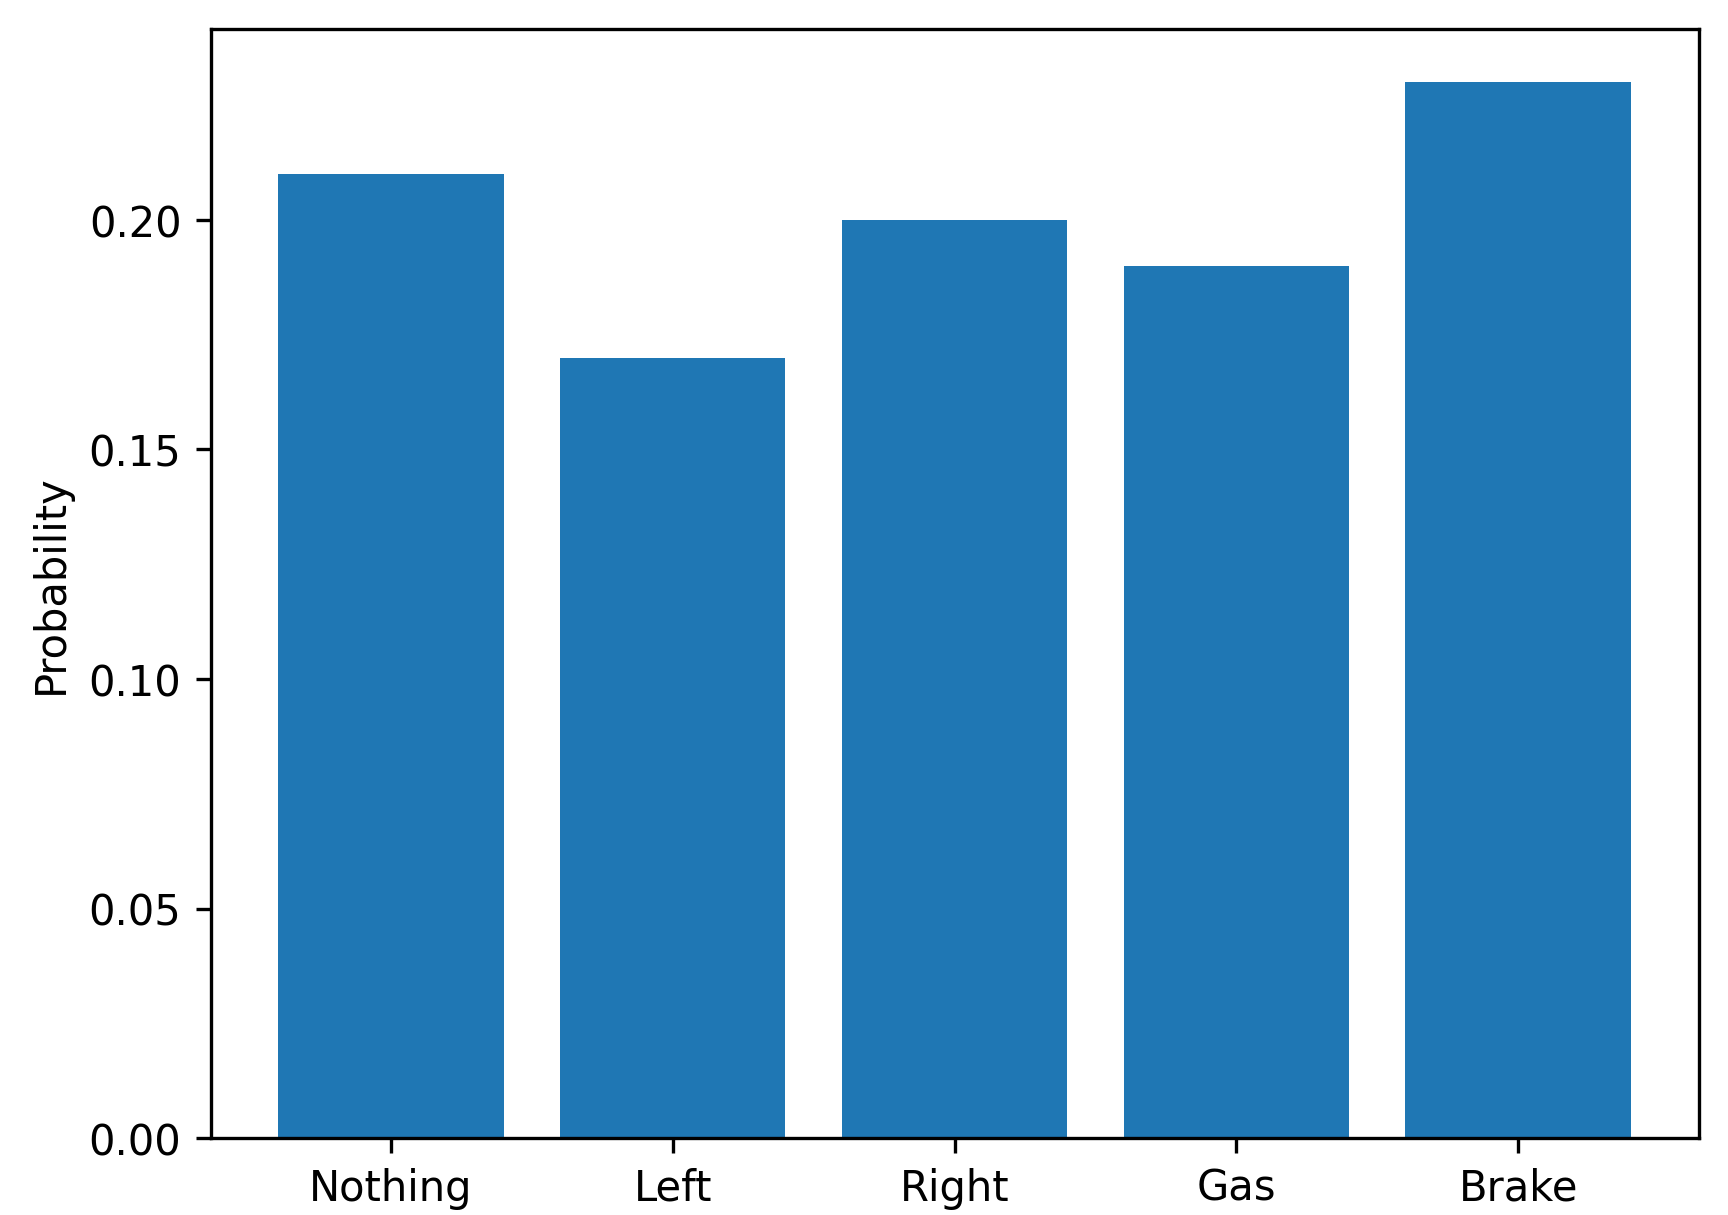
\includegraphics[height=5cm]{figures/images/regularized.png}}
    \caption{With regularization}
  \end{subfigure}
  \caption[Entropy regularization graphs]{Example of entropy regularization actor output for Car Racing}
  \label{fig:entropy_regularization}
\end{figure}


Below, we have the pseudocode for the advantage actor-critic algorithm with
entropy regularization.

\begin{algorithm}[H]
  \caption[Advantage Actor-Critic]{Advantage Actor-Critic with Entropy Regularization}
  \label{alg:advantage_actor_critic}
  \begin{algorithmic}
    \State Initialize actor network with random weights $\theta_{actor}$
    \State Initialize critic network with random weights $\theta_{critic}$
    \For{episode $i$ in $1:N$}
    \State Set initial state $s_t$
    \While{$s_t$ is not terminal}
    \State Select action $a_t$ from policy $\pi_{\theta_{actor}}(a_t~|~s_t)$ using weighted random sampling
    \State Take action $a_t$ and observe reward $r_t$ and new state $s_{t+1}$
    \State Compute advantage $A(s_t, a_t) \gets r_t+\gamma\cdot V(s_{t+1}) - V(s_t)$
    \State Compute entropy $H_t\gets-\log(\pi(a_t~|~s_t)) \cdot \pi(a_t~|~s_t)$
    \State Perform gradient descent on $-\log (\pi(a_t~|~s_t)) \cdot A(s_t, a_t) - \beta\cdot H_t$
    \State \hspace{1cm} wrt. the actor network weights $\theta_{actor}$ and update network
    \State Perform gradient descent on $A(s_t, a_t)^2$
    \State \hspace{1cm} wrt. the critic network weights $\theta_{critic}$ and update network
    \State Update state $s_t \gets s_{t+1}$
    \EndWhile
    \EndFor
  \end{algorithmic}
\end{algorithm}


\section{Agents}

This section outlines the implementation details of the agents, and it includes
the design of the neural networks; they have been implemented in Python 3.7
exactly as described in \autoref{alg:deep_q_learning} and
\autoref{alg:advantage_actor_critic}.

The network structure was not the basis of experimentation, so it was kept
relatively constant during the evaluation process. Model architectures were
inspired and adapted from other applications with similar input and output
structures.

The networks used in this project were trained using the "Adam" gradient
descent optimizer, as it has been shown to outperform alternative methods such
as stochastic gradient descent (SGD) and RMSProp \cite{kingma2014adam}.

\subsection{Mountain Car}

\subsubsection{Neural Networks}
Data is received from the environment, and it is inputted directly into the
dense (fully connected) layers of the neural network. For Mountain Car, three
layers were used for the Q-network and actor network, and two layers were used
for the critic network. We can see the networks' details in the tables below.

\begin{table}[H]
  \centering
  \begin{tabular}{|c|c|c|c|c|c|c|}
    \hline
    \textbf{Layer} & \textbf{Input} & \textbf{Activation} & \textbf{Output} \\
    \hline
    Dense          & 2              & ReLU                & 32              \\
    Dense          & 32             & ReLU                & 64              \\
    Dense          & 64             & ReLU                & 3               \\
    \hline
  \end{tabular}
  \caption[Mountain Car DQN structure]{Mountain Car deep Q-network layers and parameters}
  \label{table:mountain_car_dqn}
\end{table}


\begin{table}[H]
  \centering
  \subfloat[Actor]{
    \begin{tabular}{|c|c|c|c|c|c|c|}
      \hline
      \textbf{Layer} & \textbf{Input} & \textbf{Activation} & \textbf{Output} \\
      \hline
      Dense          & 2              & ReLU                & 32              \\
      Dense          & 32             & ReLU                & 64              \\
      Dense          & 64             & ReLU                & 3               \\
      \hline
    \end{tabular}
  }
  \subfloat[Critic]{
    \begin{tabular}{|c|c|c|c|c|c|c|}
      \hline
      \textbf{Layer} & \textbf{Input} & \textbf{Activation} & \textbf{Output} \\
      \hline
      Dense          & 2              & ReLU                & 32              \\
      Dense          & 32             & ReLU                & 1               \\
      \hline
    \end{tabular}
  }
  \caption[Mountain Car A2C network structure]{Mountain Car advantage actor-critic layers and parameters}
  \label{table:mountain_car_a2c}
\end{table}


\subsubsection{Reward Shaping} \label{sec:reward_shaping}

The Mountain Car environment has sparse rewards, so it benefits greatly in
terms of training performance to shape the reward function during training. The
same idea cannot be applied to Car Racing, as we only have access to an image
of the current frame. For this reason, we apply reward shaping in Mountain Car
to improve training speed and final scores.

In Mountain Car, the agent receives a reward of -1 for every timestep, without
any indication on performance until the episode is finished, or the goal is
reached. This means that learning is greatly diminished, as the agent can not
learn anything meaningful in the timesteps before the end of the episode. To
combat this issue, we can use reward shaping to guide the agent towards the
goal. We define a reward shaping function as shown in
\autoref{lst:reward_shaping}.

\begin{lstlisting}[style=codestyle, basicstyle=\ttfamily\footnotesize, caption={Mountain Car reward shaping}, label=lst:reward_shaping]
def shape_reward(state, next_state, reward):
  return reward + 300 * (abs(next_state[1]) - abs(state[1]))
\end{lstlisting}


This reward function takes into account the speed of the car before and after
the action, \lstinline{state[1]} and \lstinline{next_state[1]} respectively. By
adding the scaled difference in speed to the reward, the agent is incentivized
to gain more speed than had previously. The multiplier value 300 was found to
produce the highest scores after training.

\subsection{Car Racing}

\subsubsection{Frame Skipping}

A very important aspect of this environment is the idea of using a frame skip.
Without frame skipping, the frames in the frame stack are very similar as they
are consecutive, so they provide little information to the neural network about
the car's dynamics. To combat this, the agent repeats the action chosen $n + 1$
times instead of just once, and only the final state observed is added to the
frame stack. This means that consecutive images on the frame stack are further
apart in the game, and provide more information to the network about the car.
This is shown in visually \autoref{fig:frame_skip}. We can define a
\mbox{\lstinline{take_action()}} function as shown in \autoref{lst:frame_skipping}
and call this function instead of directly calling \lstinline{env.step()} in
the main episode loop for the Car Racing agents.

\begin{figure}[H]
  \centering
  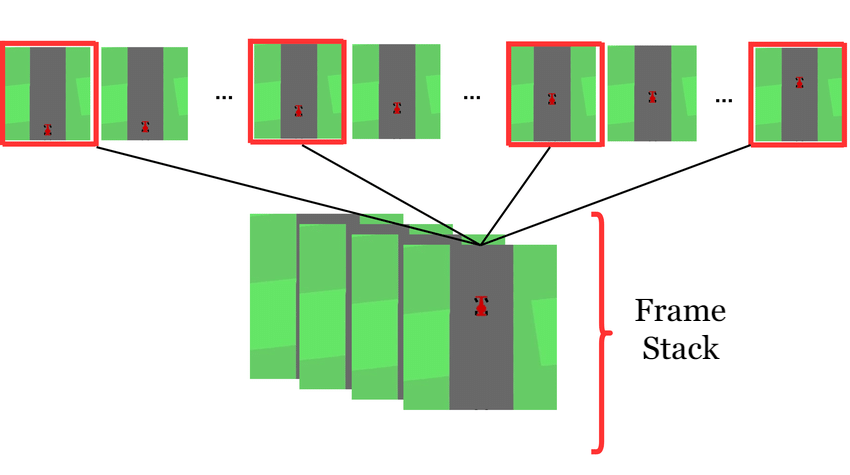
\includegraphics[width=0.75\textwidth]{figures/images/frame_skip.png}
  \caption[Car Racing frame skip]{Car Racing frame skip \cite{montoya2021decoupling}}
  \label{fig:frame_skip}
\end{figure}


\newpage

\begin{lstlisting}[style=codestyle, basicstyle=\ttfamily\footnotesize, caption={Car Racing frame skipping}, label=lst:frame_skipping]
def take_action(env, action):
  reward = 0

  for _ in range(FRAME_SKIP + 1):
      next_state, frame_reward, done, info = env.step(action)

      reward += frame_reward
      if done:
          break

  return next_state, reward, done, info
\end{lstlisting}


\subsubsection{Input Preprocessing}

For the Car Racing agent, we need to process the image before it can be passed
to the Dense layers of the network. This section is not applicable for the
Mountain Car environment, as we receive direct data about the car's position
and velocity.

The state returned by the Gym environment is a $96\times 96$ RGB image, which
contains:

\begin{itemize}
  \item A dynamically coloured car at a fixed coordinate position in the image
  \item A polychromatic gray track and green grass surrounding the track
  \item Red and white curbs on the track corners (not visible in the figure) black
  \item A "dashboard" at the bottom with metadata about the car
\end{itemize}

Most of these details are unnecessary, and would require more extensive and
complex neural networks to extract features relevant to the policy. We can
therefore process the image before passing it to the network. Below are the
steps used in this project for doing so, and their corresponding line of code
in \autoref{lst:car_racing_image_processing}. OpenCV and numpy were used for
this, as shown in the code sample.

\begin{itemize}
  \item \textbf{Desaturation} -- converts the image to greyscale reducing the
        computational load by turning a $96\times 96\times 3$ image to $96\times
          96\times 1$, without losing any necessary detail
  \item \textbf{Masking} -- draws a black box to emphasize the car and
        reduce unwanted interference from the car's details and changing colour between
        episodes
  \item \textbf{Colour homogenization} -- homogenizes the different colour shades of
        the track (including curbs) and grass, which add unnecessary complexity; these
        details are not required to find the optimal policy
  \item \textbf{Cropping} -- crops the "dashboard" area, as it is not required and adds
        an unwanted artefact to the image; the square ratio is maintained by cropping
        the sides of the image, as these areas mostly only contain grass
  \item \textbf{Normalization} -- scales pixel values to be in the range $[0, 1]$,
        helping the optimization algorithm navigate the parameter space
\end{itemize}

\newpage

\begin{lstlisting}[style=codestyle, basicstyle=\ttfamily\footnotesize, caption={Car Racing state image preprocessing}, label=lst:car_racing_image_processing]
def process_state(state):
  # Desaturation
  state = cv2.cvtColor(state, cv2.COLOR_BGR2GRAY).astype(float)

  # Masking
  cv2.rectangle(state, (45, 66), (50, 76), 0, -1)

  # Colour homogenization
  state[np.where((state >= 160) & (state < 180))] = 255
  state[np.where((state >= 90) & (state < 160))] = 100

  # Cropping
  state = state[0:84, 6:90]

  # Normalization
  state /= 255.0

  return state
\end{lstlisting}


The result of this image processing can be seen in
\autoref{fig:car_racing_state_processing}. Note that the grey border is not
part of the image passed to the neural network, and has been added for image
edge clarity.

\begin{figure}[H]
  \centering
  \begin{subfigure}{0.22\linewidth}
    {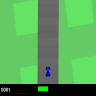
\includegraphics{figures/images/car_racing_state_original.png}}
    \caption{Original state}
  \end{subfigure}
  \qquad\tikz[baseline=-4\baselineskip]\draw[ultra thick,->] (0,0) -- ++ (1,0);\qquad
  \begin{subfigure}{0.2\linewidth}
    \fbox{
\includegraphics{figures/images/car_racing_state_processed.png}}
    \caption{Processed state}
  \end{subfigure}
  \caption[Car Racing state preprocessing]{Preprocessing of the Car Racing input state image}
  \label{fig:car_racing_state_processing}
\end{figure}


\subsubsection{Neural Networks}

Images are added to the frame stack after they have been preprocessed, and the
entire data structure is passed to the neural network. The frame stack allows
the network to deduce the car's speed and direction, as explained in
\autoref{sec:markov_property}.

The first step performed by the neural networks is a convolution with ReLU
activation, paired with a max pooling layer. This is then repeated once again
with different filter sizes, after which a flatten layer linearizes the data.
The linear data is then passed to the two dense layers of the neural network.

This structure is common across the deep Q-network and both the actor and
critic networks, with the only difference being the output size. Below are
tables with the exact parameters used in the neural networks for both
algorithms.

\begin{table}[H]
  \centering
  \subfloat{
    \small
    \begin{tabular}{|c|c|c|>{\centering\arraybackslash}p{1cm}|c|c|>{\centering\arraybackslash}p{1.5cm}|c|}
      \hline
      \textbf{Layer} & \textbf{Input}        & \textbf{Filters} & \textbf{Filter Size} & \textbf{Stride} & \textbf{Activation} & \textbf{Regular-ization} & \textbf{Output}       \\
      \hline
      Conv           & $84\times 84\times 3$ & 8                & $7\times 7$          & 4               & ReLU                & L2                       & $20\times 20\times 8$ \\
      MaxPooling     & $20\times 20\times 8$ & -                & $2\times 2$          & 2               & -                   & -                        & $10\times 10\times 8$ \\
      Conv           & $10\times 10\times 8$ & 16               & $3\times 3$          & 1               & ReLU                & L2                       & $8\times 8\times 16$  \\
      MaxPooling     & $8\times 8\times 16$  & -                & $2\times 2$          & 2               & -                   & -                        & $4\times 4\times 16$  \\
      Flatten        & $4\times 4\times 16$  & -                & -                    & -               & -                   & -                        & 256                   \\
      Dense          & 256                   & -                & -                    & -               & ReLU                & L2                       & 512                   \\
      Dense          & 512                   & -                & -                    & -               & Linear              & L2                       & 5                     \\
      \hline
    \end{tabular}
  }
  \caption[Car Racing DQN structure]{Car Racing deep Q-network layers and parameters}
  \label{table:car_racing_dqn}
\end{table}


\begin{table}[H]
  \centering
  \subfloat[Actor]{
    \small
    \begin{tabular}{|c|c|c|>{\centering\arraybackslash}p{1cm}|c|c|>{\centering\arraybackslash}p{1.5cm}|c|}
      \hline
      \textbf{Layer} & \textbf{Input}        & \textbf{Filters} & \textbf{Filter Size} & \textbf{Stride} & \textbf{Activation} & \textbf{Regular-ization} & \textbf{Output}       \\
      \hline
      Conv           & $84\times 84\times 3$ & 8                & $7\times 7$          & 4               & ReLU                & L2                       & $20\times 20\times 8$ \\
      MaxPooling     & $20\times 20\times 8$ & -                & $2\times 2$          & 2               & -                   & -                        & $10\times 10\times 8$ \\
      Conv           & $10\times 10\times 8$ & 16               & $3\times 3$          & 1               & ReLU                & L2                       & $8\times 8\times 16$  \\
      MaxPooling     & $8\times 8\times 16$  & -                & $2\times 2$          & 2               & -                   & -                        & $4\times 4\times 16$  \\
      Flatten        & $4\times 4\times 16$  & -                & -                    & -               & -                   & -                        & 256                   \\
      Dense          & 256                   & -                & -                    & -               & ReLU                & L2                       & 512                   \\
      Dense          & 512                   & -                & -                    & -               & Linear              & L2                       & 5                     \\
      \hline
    \end{tabular}
  }
  \vspace{0.8cm}
  \subfloat[Critic]{
    \small
    \begin{tabular}{|c|c|c|>{\centering\arraybackslash}p{1cm}|c|c|>{\centering\arraybackslash}p{1.5cm}|c|}
      \hline
      \textbf{Layer} & \textbf{Input}        & \textbf{Filters} & \textbf{Filter Size} & \textbf{Stride} & \textbf{Activation} & \textbf{Regular-ization} & \textbf{Output}       \\
      \hline
      Conv           & $84\times 84\times 3$ & 8                & $7\times 7$          & 4               & ReLU                & L2                       & $20\times 20\times 8$ \\
      MaxPooling     & $20\times 20\times 8$ & -                & $2\times 2$          & 2               & -                   & -                        & $10\times 10\times 8$ \\
      Conv           & $10\times 10\times 8$ & 16               & $3\times 3$          & 1               & ReLU                & L2                       & $8\times 8\times 16$  \\
      MaxPooling     & $8\times 8\times 16$  & -                & $2\times 2$          & 2               & -                   & -                        & $4\times 4\times 16$  \\
      Flatten        & $4\times 4\times 16$  & -                & -                    & -               & -                   & -                        & 256                   \\
      Dense          & 256                   & -                & -                    & -               & ReLU                & L2                       & 512                   \\
      Dense          & 512                   & -                & -                    & -               & Linear              & L2                       & 1                     \\
      \hline
    \end{tabular}
  }
  \caption[Car Racing A2C network structure]{Car Racing advantage actor-critic layers and parameters}
  \label{table:car_racing_a2c}
\end{table}


\newpage

\section{Visualization} \label{sec:visualization_design}
As this project was coded in Python using Tensorflow 2, there were a couple
options considered for the visualization. The first was a web based GUI using
Tensorflow.js, although this would have required an emulation system to be able
to see the gameplay in the browser, making it a needlessly complicated option.

The method implemented for this project was a Tkinter\footnote{Tkinter is a
  Python standard library GUI toolkit} based GUI. In order to make the user
interface look modern, we used the Ttk styling module, which is included in the
standard Tkinter installation.

The GUI consists of two modes for each of the game-algorithm pairs: gameplay
visualization, allowing the user to view the chosen agent play an episode of
the chosen game with a model that has been trained for a specified number of
episodes; and model/reward visualization, which shows the user the progression
of the model's weights and biases as training progresses, alongside a reward
graph. \autoref{fig:gui} shows the main menu of the GUI, where the user can
select the aforementioned visualization modes.

\begin{figure}[H]
  \centering
  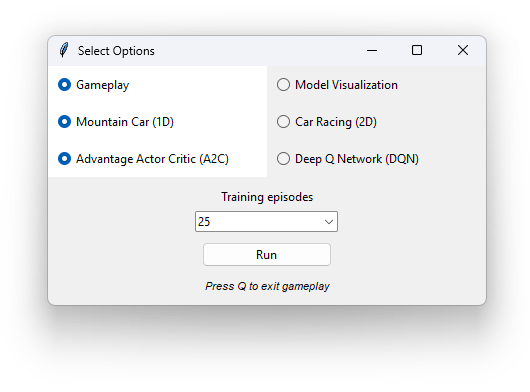
\includegraphics[width=0.45\textwidth]{figures/images/gui.png}
  \caption[Visualization GUI]{Graphical user interface for accessing the visualization suite}
  \label{fig:gui}
\end{figure}


In \autoref{fig:mountain_car_gui}, we can see the visualizations for Mountain
Car. On the left, have a visualization of the reward history graph with a
slider to control the rolling average window size. On the right, we have both a
weight distribution histogram and node connection graph side by side. The
slider below controls which model to use for the graphs, based on the number of
training episodes.

\autoref{fig:car_racing_gui} shows the Car Racing visualization GUI. Similarly to the Mountain Car visualization, we have a reward history graph. This works in exactly the same way as described above, as it is using the same runner file to load the GUI, with different data. The difference lies in the model visualization, where we can see the filters of the first layer of the CNN instead.

The GUI dynamically updates to reflect the changes in the graphs when either of
the sliders is used.

\begin{figure}[H]
  \centering
  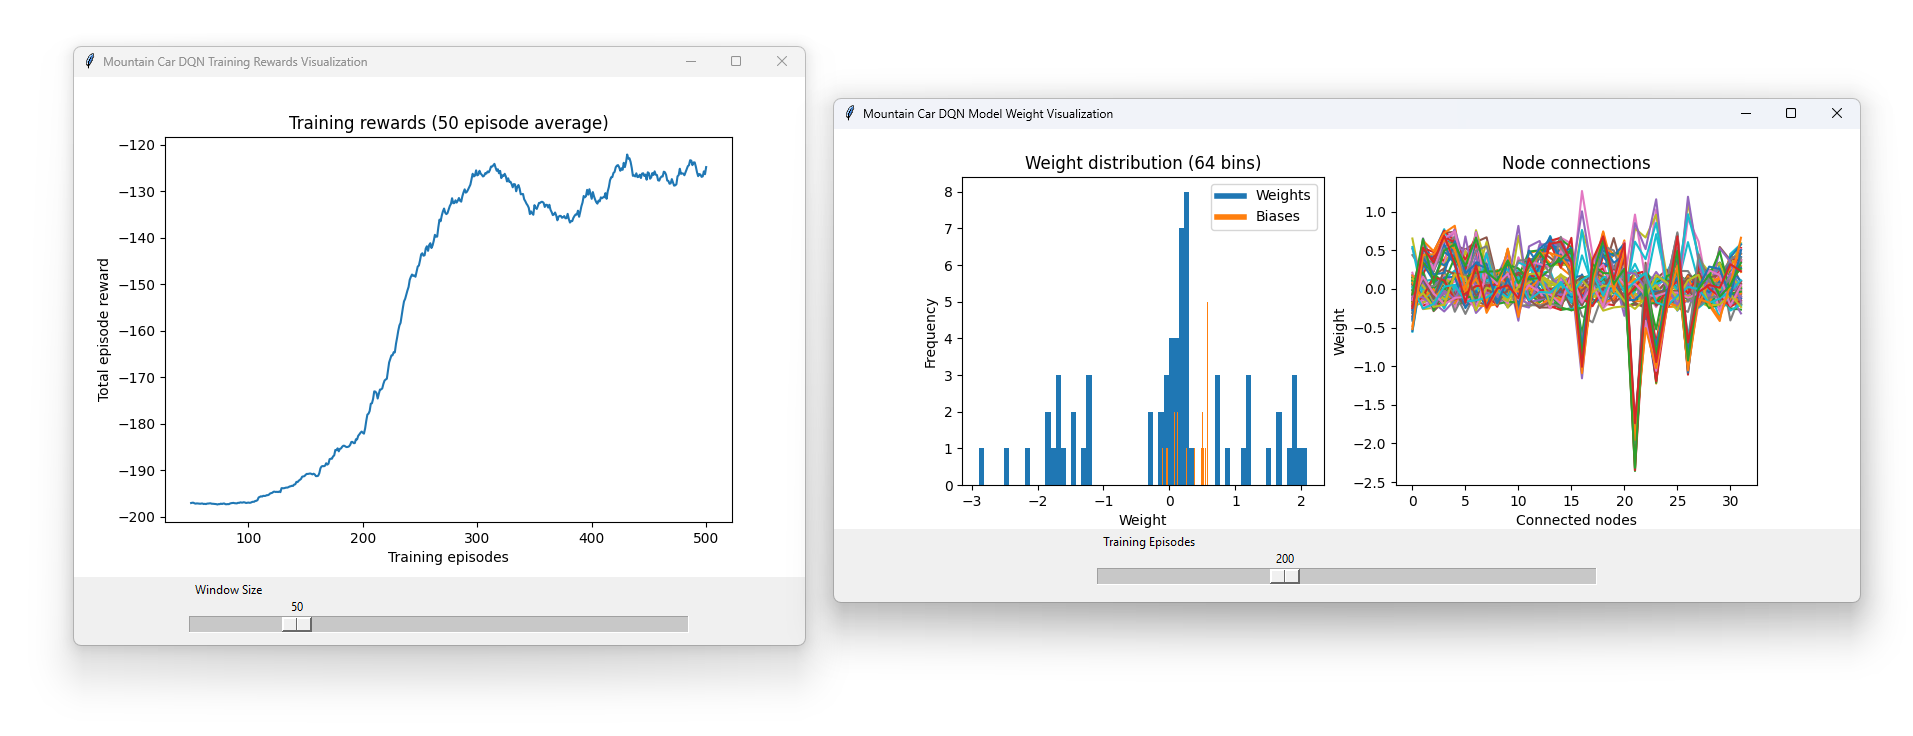
\includegraphics[width=1\textwidth]{figures/images/mountain_car_gui.png}
  \caption[Mountain Car DQN model visualization GUI]{Model visualization GUI for Mountain Car DQN}
  \label{fig:mountain_car_gui}
\end{figure}


\begin{figure}[H]
  \centering
  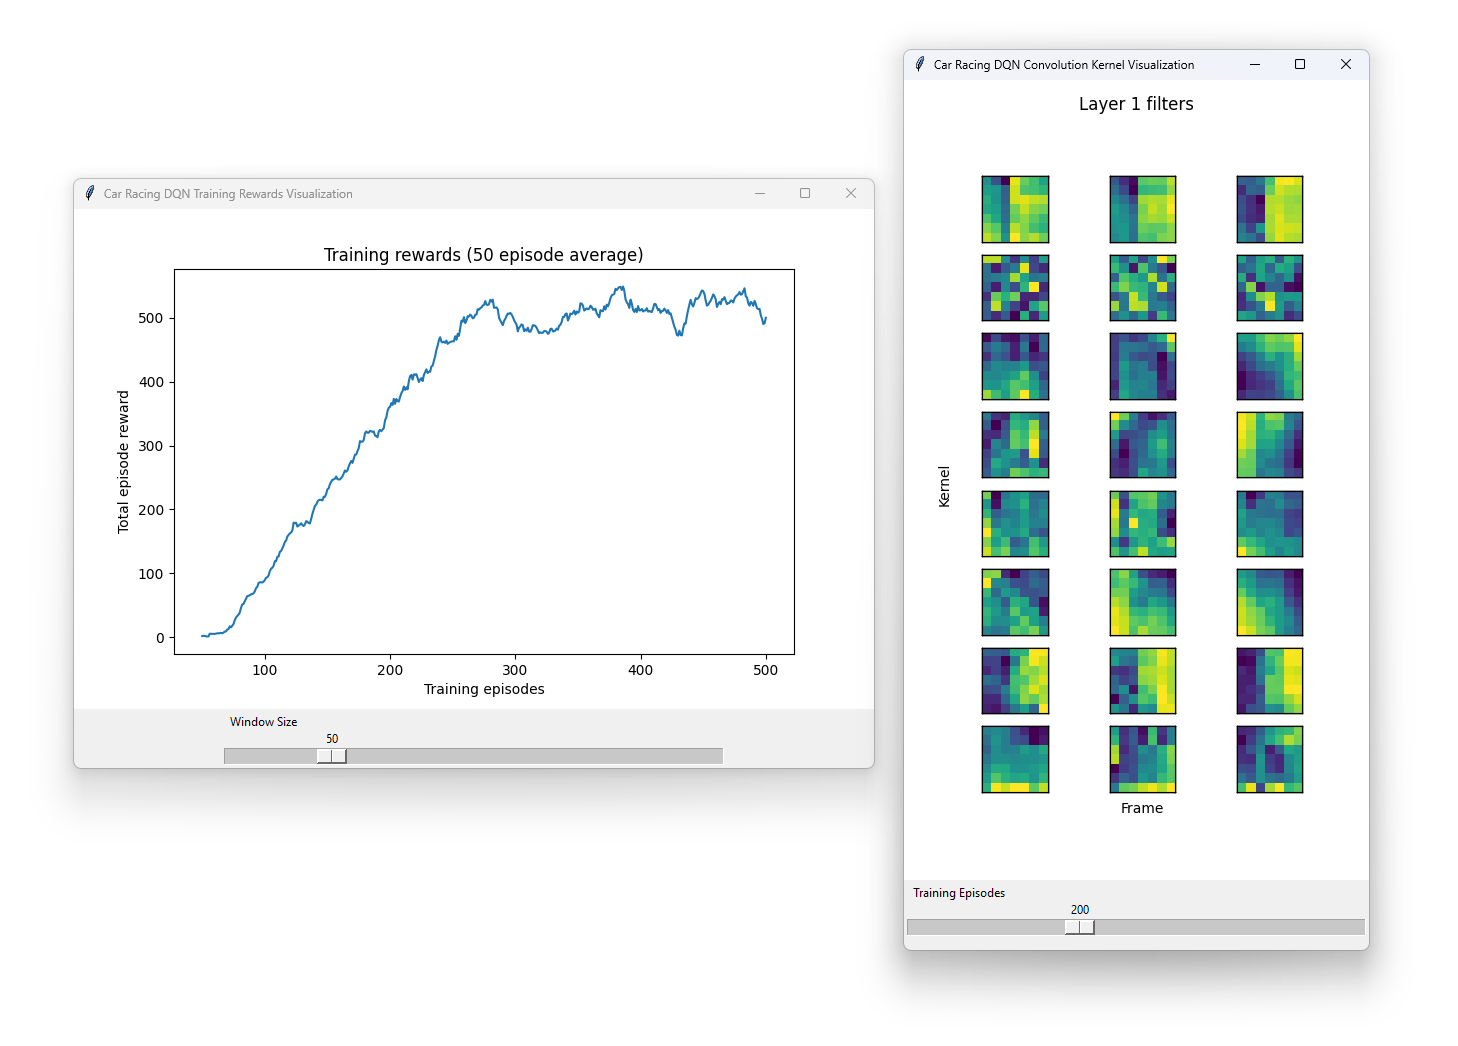
\includegraphics[width=0.8\textwidth]{figures/images/car_racing_gui.png}
  \caption[Car Racing DQN model visualization GUI]{Model visualization GUI for Car Racing DQN}
  \label{fig:car_racing_gui}
\end{figure}

